\documentclass{article}
%\usepackage{tex4ht}
\usepackage{amsmath}
\usepackage{amsfonts}
\usepackage{amssymb}
\usepackage{amsthm}
\usepackage{graphicx}
\usepackage{color}
\usepackage{float}
\usepackage{dsfont}
\setlength{\parskip}{0.5\baselineskip}
\author{Zhuo Liu (0983311)}
\title{Project on Automatic Learning (Phase 2, Part 2)}
\date{February 25, 2014}

\definecolor{lightgray}{gray}{0.5}


\begin{document}
\maketitle


\section{Introduction}

In this report, we will first use the data obtained by PCA from Part 1, and linear discriminant analysis (LDA) to build a linear classifier on the
feature space. We will test the classifier by checking the accuracy on both training and test set. Then, we will apply kernel PCA to the same data
set again, to obtain a KPC space, and also apply LDA on this KPC space to build a classifier. Since kernel PCA is nonlinear, the
classifier we build will be also a nonlinear classifier. In particular, the kernel we use in KPCA will be Gaussian Kernel, i.e.
\begin{equation}
 k(x,y) = exp(-\frac{||x-y||^{2}}{2\sigma^{2}}).
\end{equation}
Still, the accuracy on both training and test set will be provided, and we can compare the result to the one by first linear classifier.

%%% ------------------------------------------------------------------------------
\goodbreak

\section{Database: the Large One}

\subsection{Linear Classifier}

First we check the accuracy of the classifier build from LDA on the principle components space. The requirement of the PC space is that 
90 percent of energy will be kept, i.e. we will keep k largest eigenvalues of covariance matrix, s.t.
\begin{equation}
 \frac{\sum_{i=1}^{k}\lambda_{i}}{\sum_{i=1}^{256}\lambda_{i}} > 0.9
\end{equation}

In order to see how the size of training set affects on the accuracy, we randomly choose training sets 9 times, whose sizes are $10\%$,$20\%$,...,$90\%$ 
of whole data set, and the remaining data compose the test set. The following table shows the accuracy of the linear classifier (Here, when the size
of training set is $10\%$, the result is not available. The reason is there will be more descriptors than obeservations, so PCA cannot be applied):

\scalebox{0.9}{
 \begin{tabular}{|c|c|c|c|}
  \hline
  Size of Traing Set  & Number of PCs  & Acc. on Training Set & Acc. on Test Set \\ \hline
  $10\%$              & N/A            & N/A                  & N/A              \\ \hline
  $20\%$              & 82             & 0.9842767            & 0.8541176        \\ \hline
  $30\%$              & 92             & 0.9769392            & 0.8772401        \\ \hline
  $40\%$              & 98             & 0.9670330            & 0.8891213        \\ \hline
  $50\%$              & 102            & 0.9585427            & 0.8946048        \\ \hline
  $60\%$              & 104            & 0.9591623            & 0.8855799        \\ \hline
  $70\%$              & 106            & 0.9551570            & 0.9058577        \\ \hline
  $80\%$              & 108            & 0.9466248            & 0.9122257        \\ \hline
  $90\%$              & 109            & 0.9469644            & 0.8937500        \\ \hline
 \end{tabular}
}
 
Figure 1,2,3 show the data projected on the first two, second two and third two LD components space:

\begin{figure}[htp]
\centering
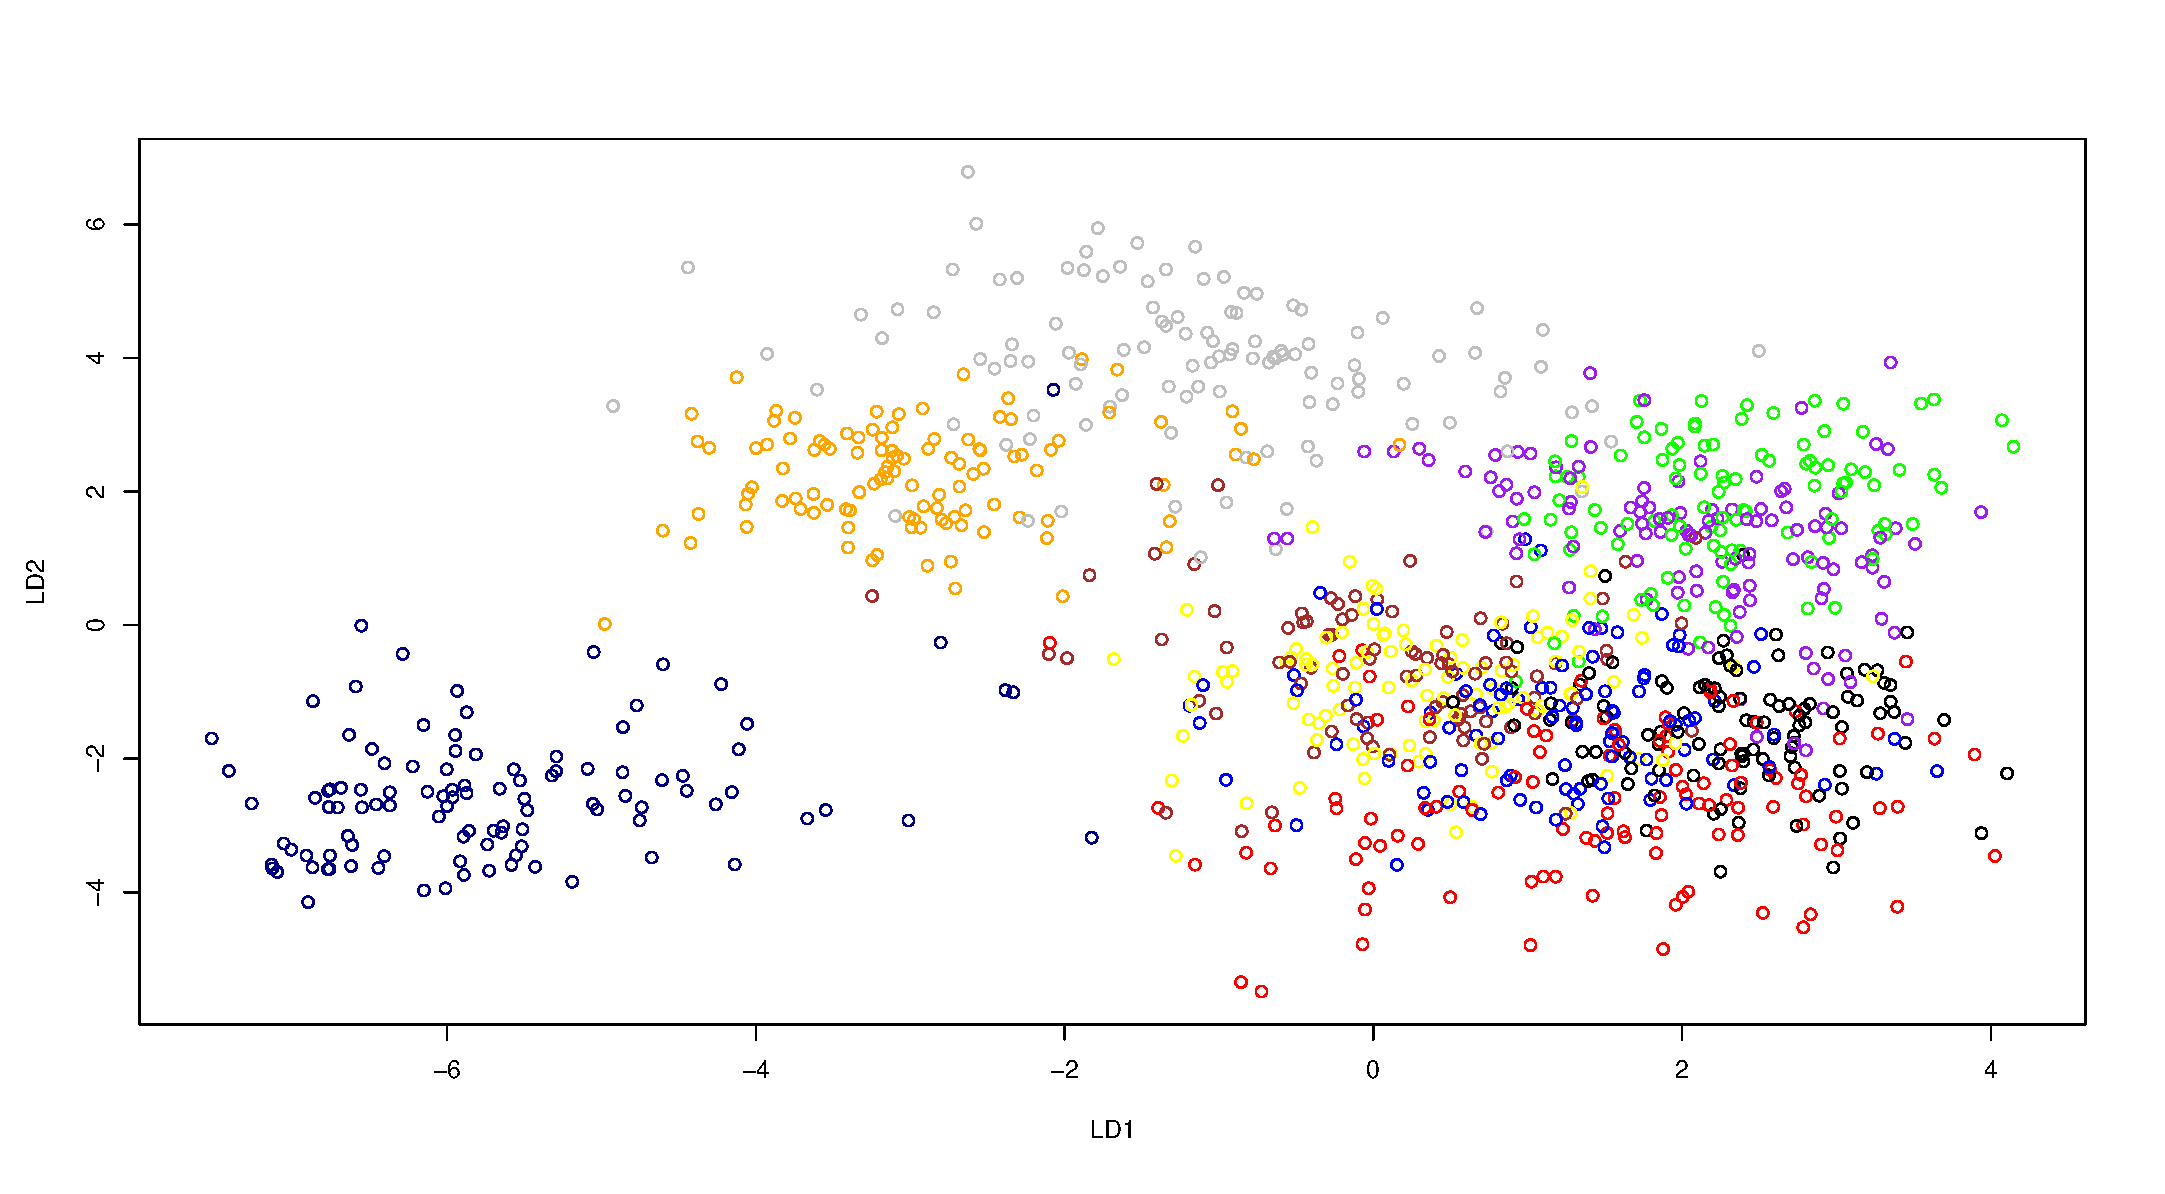
\includegraphics[width=12.1cm]{large_pcalda_LD12_train.eps}
\caption{\textit{Projection of PC space onto first two LD componets space (large data set). Here, the colors represent different classes: navy--0, green--1, 
blue--2, black--3, grey--4, brown--5, orange--6, purple--7, yellow--8, red--9.}}
\end{figure}

\begin{figure}[htp]
\centering
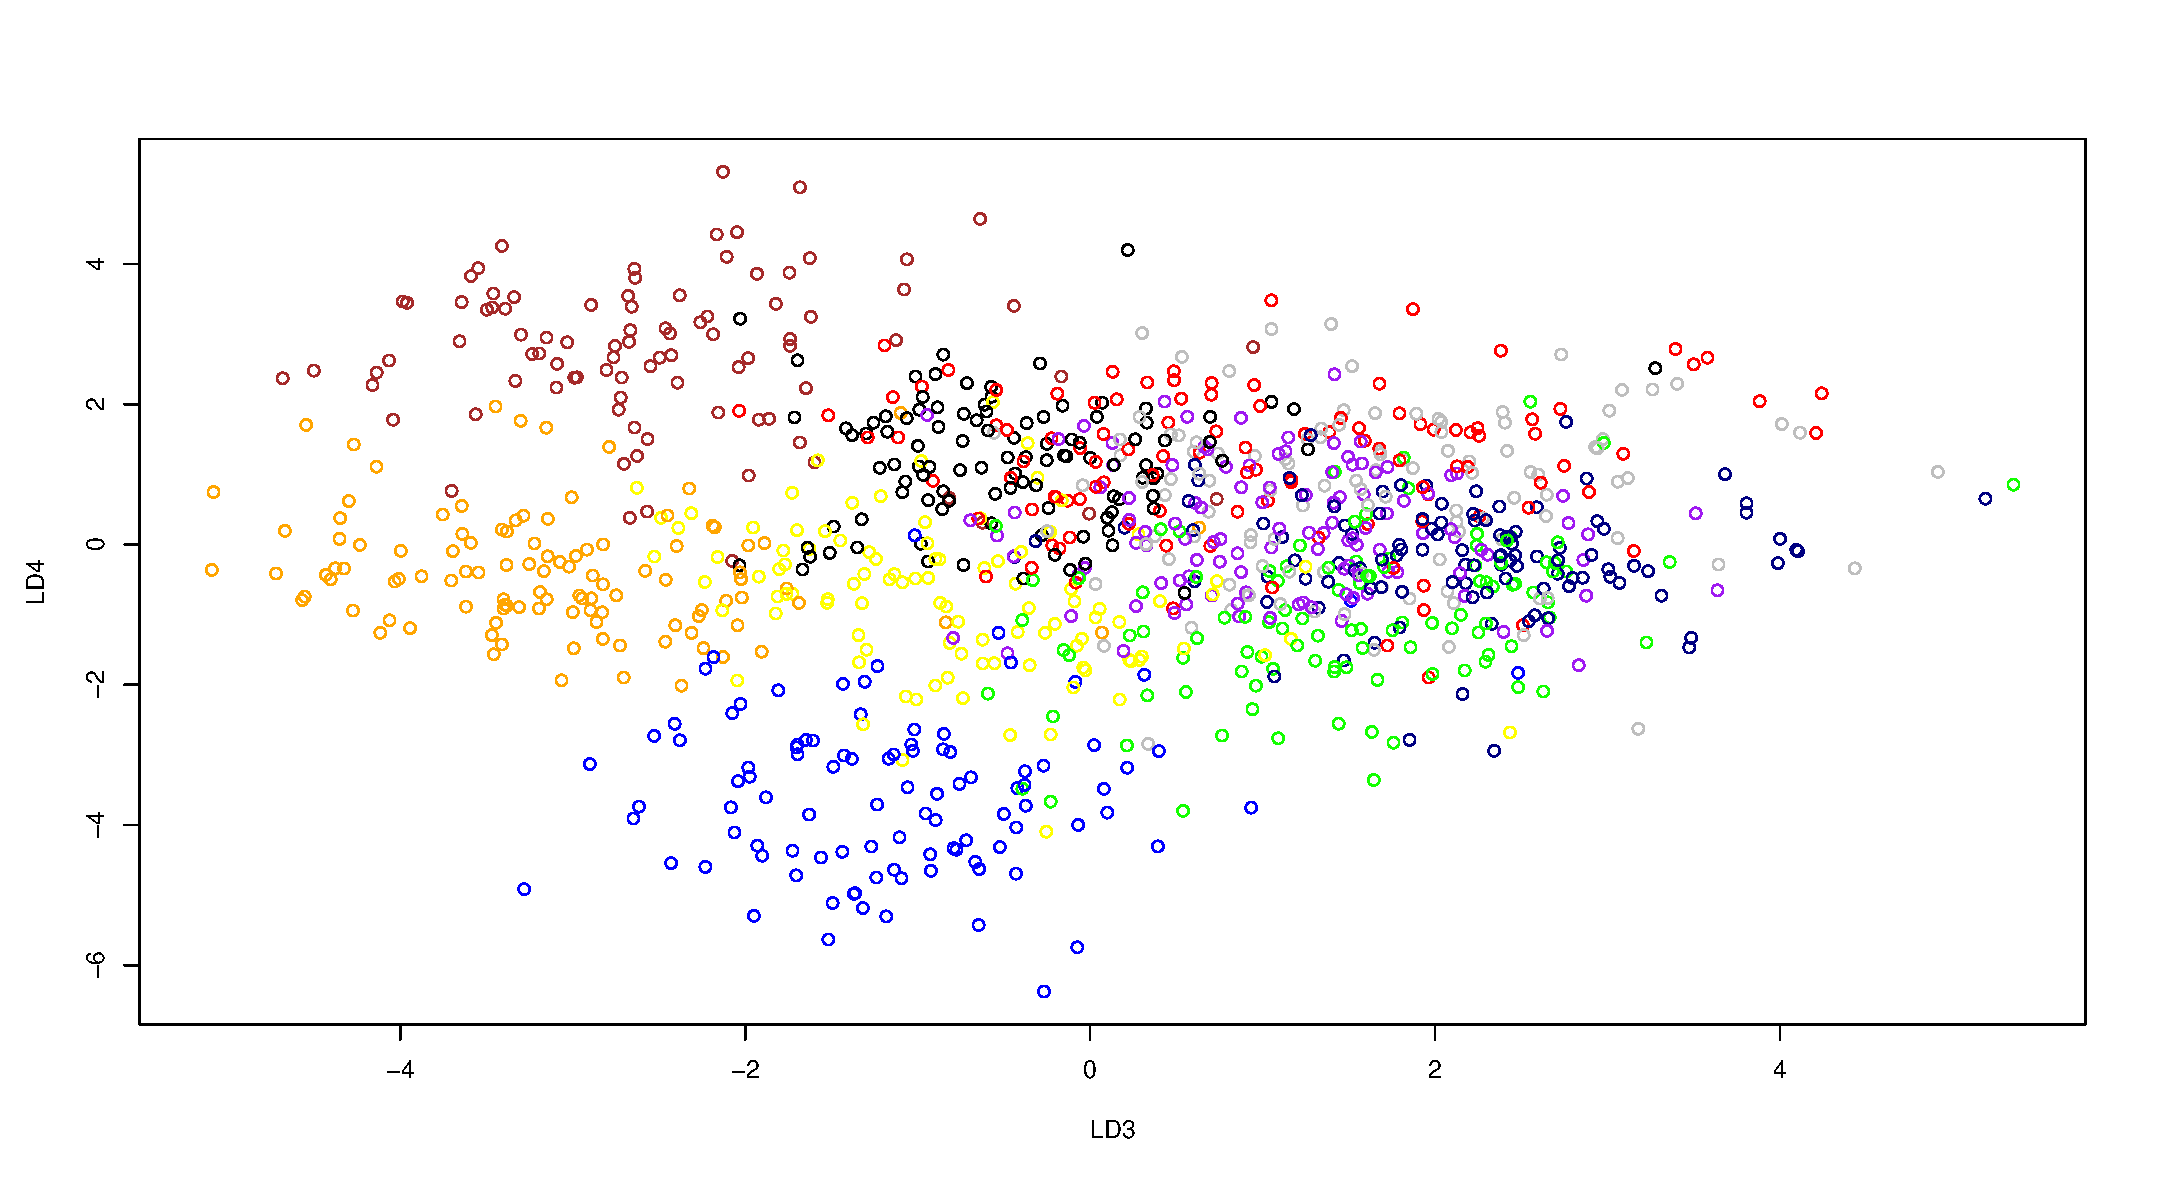
\includegraphics[width=12.1cm]{large_pcalda_LD34_train.eps}
\caption{\textit{Projection of PC space onto second two LD components space (large data set). Here, the colors represent different classes: navy--0, green--1, 
blue--2, black--3, grey--4, brown--5, orange--6, purple--7, yellow--8, red--9.}}
\end{figure}

\begin{figure}[htp]
\centering
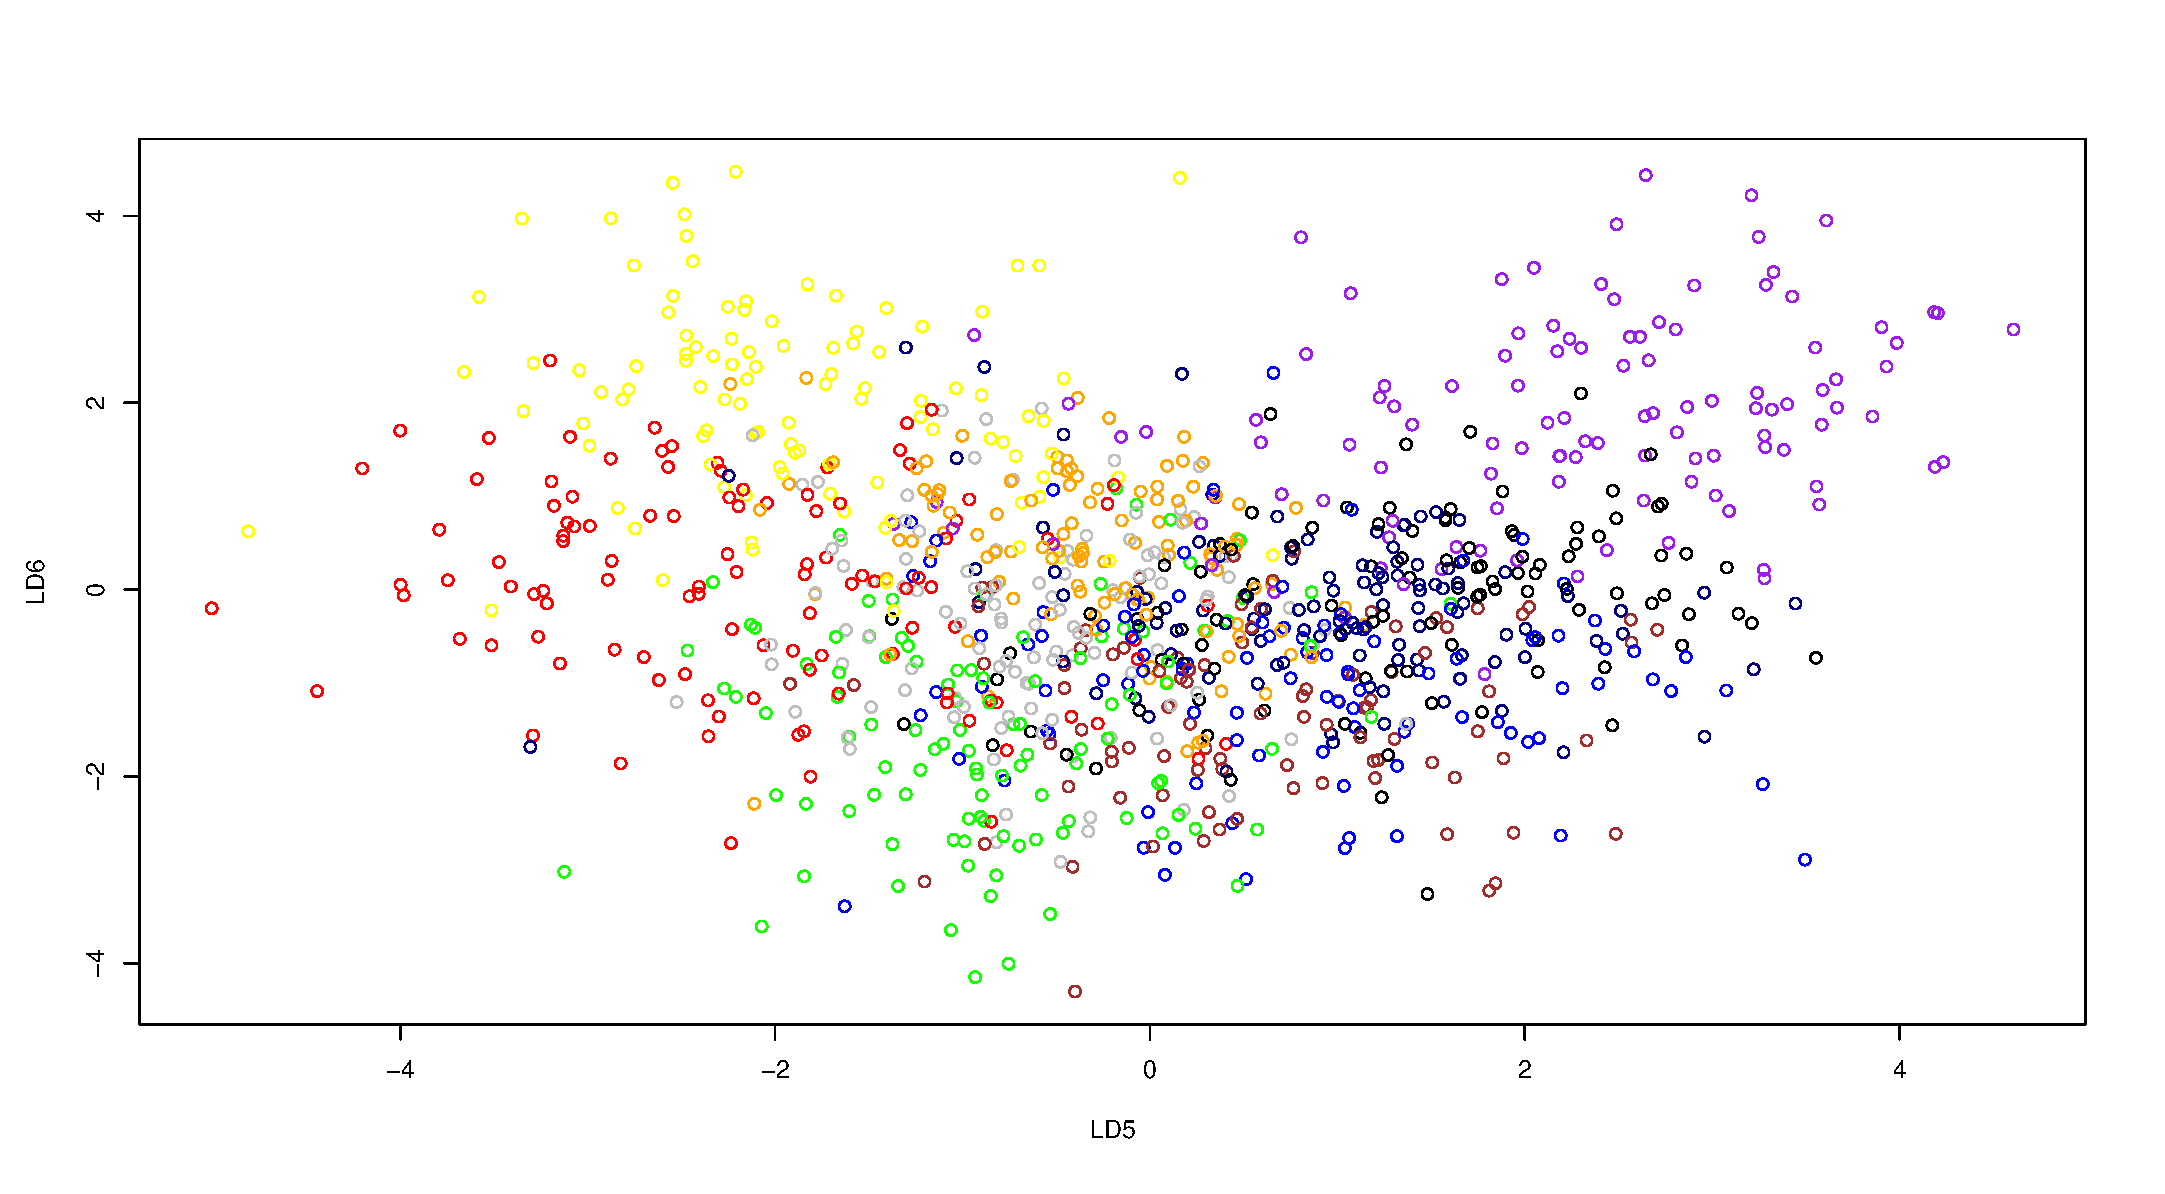
\includegraphics[width=12.1cm]{large_pcalda_LD56_train.eps}
\caption{\textit{Projection of PC space onto third two LD components space (large data set). Here, the colors represent different classes: navy--0, green--1, 
blue--2, black--3, grey--4, brown--5, orange--6, purple--7, yellow--8, red--9.}}
\end{figure}

It is not difficult to find that obeservations in different classes are not well seperated, so it is impossible to build a very good linear classifier.

\newpage

\subsection{Nonlinear Classifier}

Next, we will also use LDA to build a classifier, but now, on the kernel PC space. It will be a nonlinear classifier on the original feature space. 
By several experiment, the optimal parameter $\sigma$ in Gaussion kernel function is $\sigma=6.455$. The following table shows the result:

\scalebox{0.88}{
 \begin{tabular}{|c|c|c|c|}
  \hline
  Size of Traing Set  & Number of KPCs & Acc. on Training Set & Acc. on Test Set \\ \hline
  $10\%$              & 118            & 1                    & 0.8026499        \\ \hline
  $20\%$              & 222            & 1                    & 0.8847059        \\ \hline
  $30\%$              & 320            & 1                    & 0.9094982        \\ \hline
  $40\%$              & 416            & 1                    & 0.9476987        \\ \hline
  $50\%$              & 505            & 1                    & 0.9560853        \\ \hline
  $60\%$              & 588            & 1                    & 0.9514107        \\ \hline
  $70\%$              & 667            & 1                    & 0.9623431        \\ \hline
  $80\%$              & 726            & 1                    & 0.9655172        \\ \hline
  $90\%$              & 759            & 1                    & 0.9625000        \\ \hline
 \end{tabular}
}

Figure 4,5 show the data projected on the first two and second two LD components space:

\begin{figure}[htp]
\centering
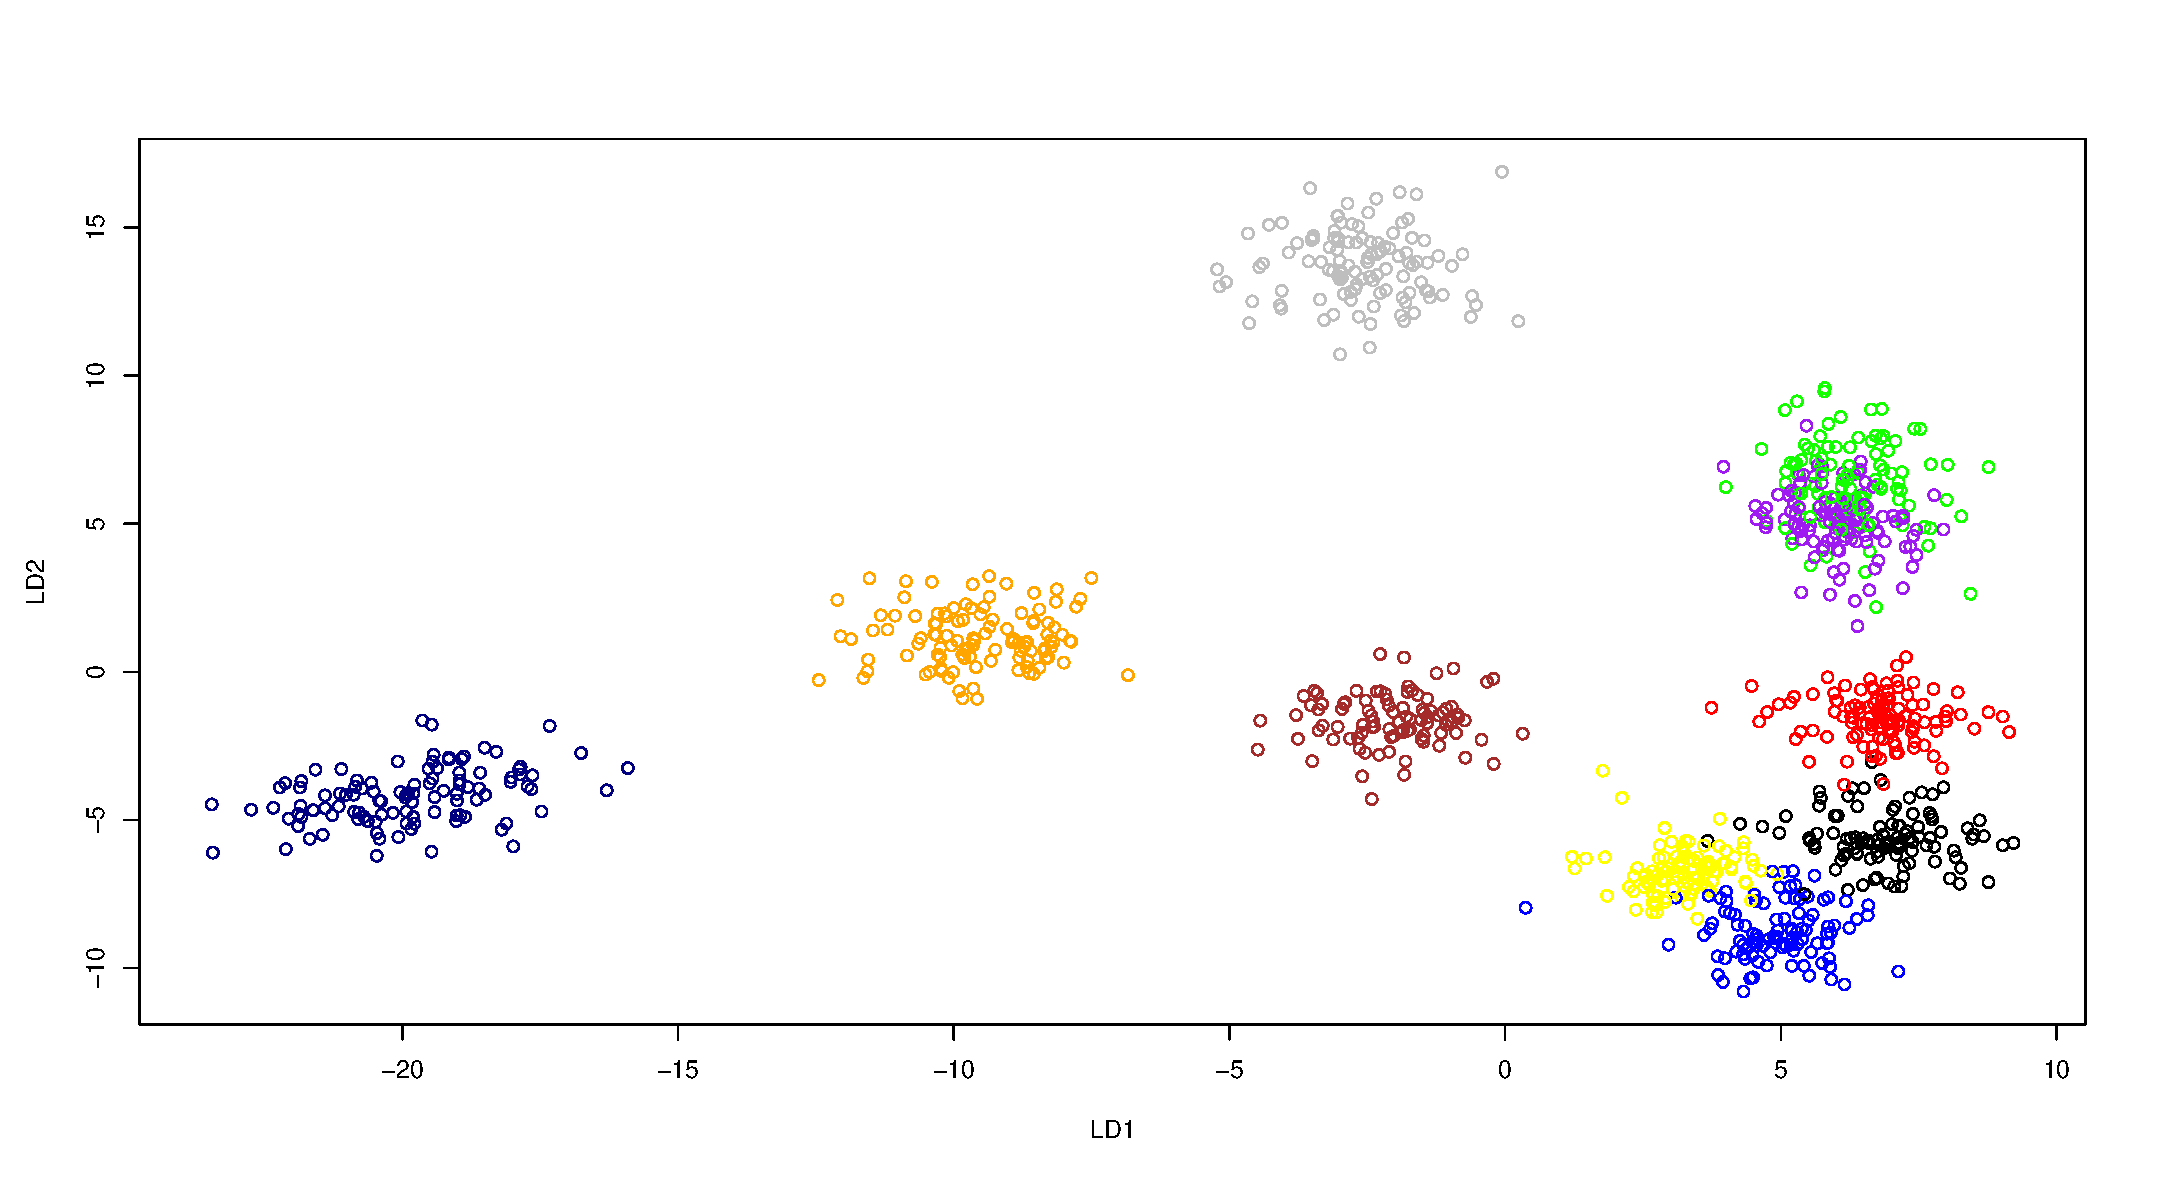
\includegraphics[width=12.1cm]{large_kpcalda_LD12_train.eps}
\caption{\textit{Projection of KPC space onto first two LD components space (large data set). Here, the colors represent different classes: navy--0, green--1, 
blue--2, black--3, grey--4, brown--5, orange--6, purple--7, yellow--8, red--9.}}
\end{figure}

\begin{figure}[htp]
\centering
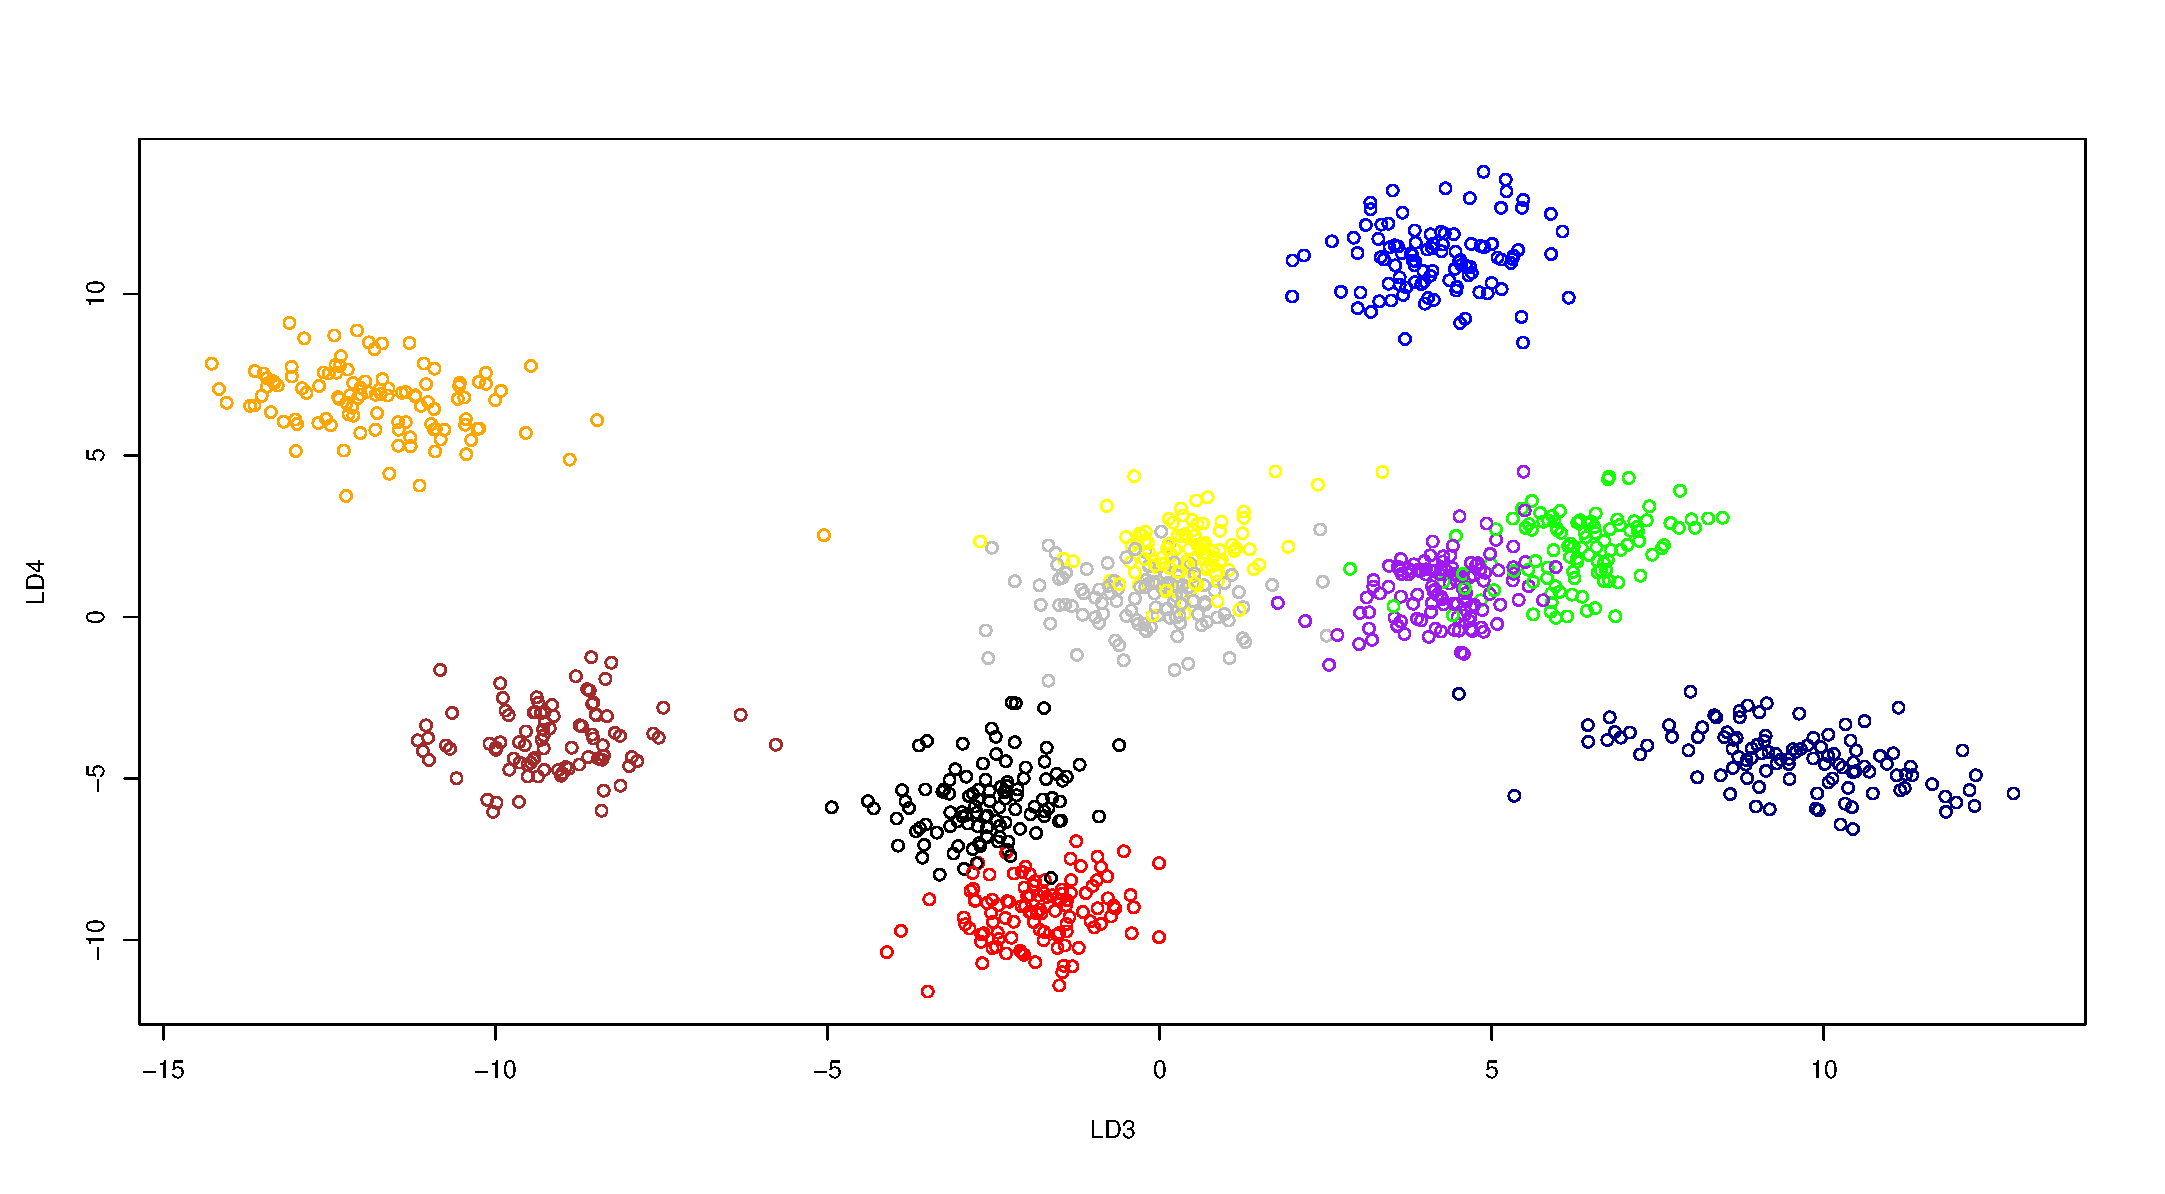
\includegraphics[width=12.1cm]{large_kpcalda_LD34_train.eps}
\caption{\textit{Projection of KPC space onto second two LD components space (large data set). Here, the colors represent different classes: navy--0, green--1, 
blue--2, black--3, grey--4, brown--5, orange--6, purple--7, yellow--8, red--9.}}
\end{figure}

By doing kernel trick, the obeservations in different classes are well separated, and we can easily build a linear classifier on this space.
This explains why the result for this nonlinear classifier performs much better than the linear classifier build on PC space.

%%% ------------------------------------------------------------------------------
\goodbreak

\section{Database: the Small One}

\subsection{Linear Classifier}

Similar to the procedure for large data set, first we build a linear classifier from the PC space which keeps $90\%$ of energy, the following table
shows the accuracy:

\scalebox{0.9}{
 \begin{tabular}{|c|c|c|c|}
  \hline
  Size of Traing Set  & Number of PCs  & Acc. on Training Set & Acc. on Test Set \\ \hline
  $10\%$              & 3              & 0.7878788            & 0.7638288        \\ \hline
  $20\%$              & 4              & 0.7748918            & 0.7754329        \\ \hline
  $30\%$              & 4              & 0.7878788            & 0.7835498        \\ \hline
  $40\%$              & 4              & 0.7846320            & 0.7886003        \\ \hline
  $50\%$              & 4              & 0.7844156            & 0.7913420        \\ \hline
  $60\%$              & 4              & 0.7813853            & 0.7889610        \\ \hline
  $70\%$              & 4              & 0.7903525            & 0.7676768        \\ \hline
  $80\%$              & 4              & 0.7911255            & 0.7597403        \\ \hline
  $90\%$              & 4              & 0.7883598            & 0.7532468        \\ \hline
 \end{tabular}
}
 
Fiugre 6,7 shows the data projected on the first two and second two LD components space. From these two figures, we can find that it is even more 
difficult to seperate the data in this PC space than those in large database, so the accuracy is very low.

\begin{figure}[htp]
\centering
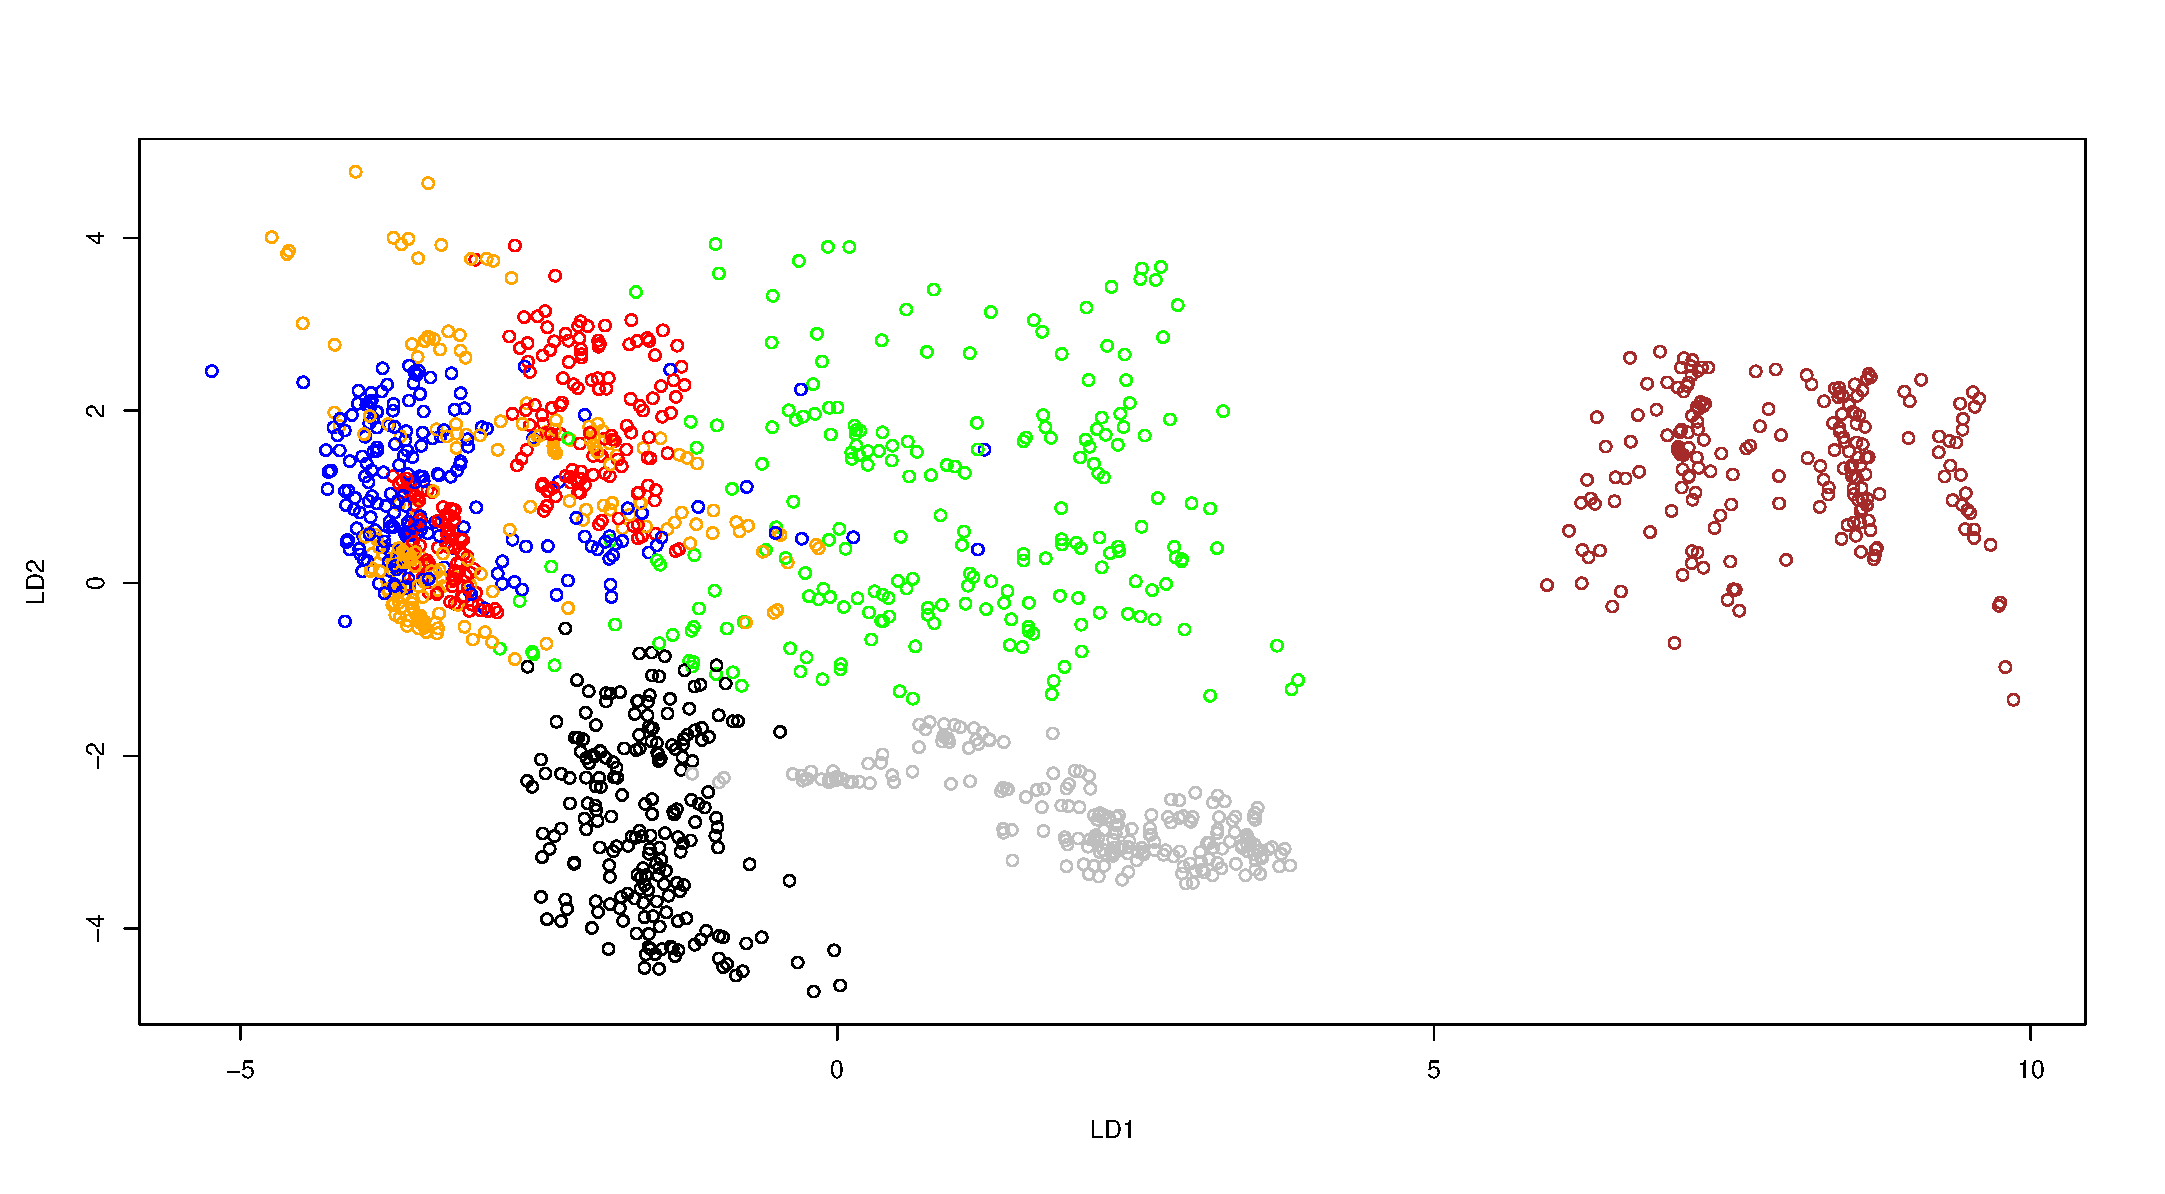
\includegraphics[width=12.1cm]{small_pcalda_LD12_train.eps}
\caption{\textit{Projection of PC space onto first two LD componets space (small data set). Here, the colors represent different classes: red--brickface, brown--sky, 
blue--foliage, green--cement, orange--window, grey--path, black--grass.}}
\end{figure}

\begin{figure}[htp]
\centering
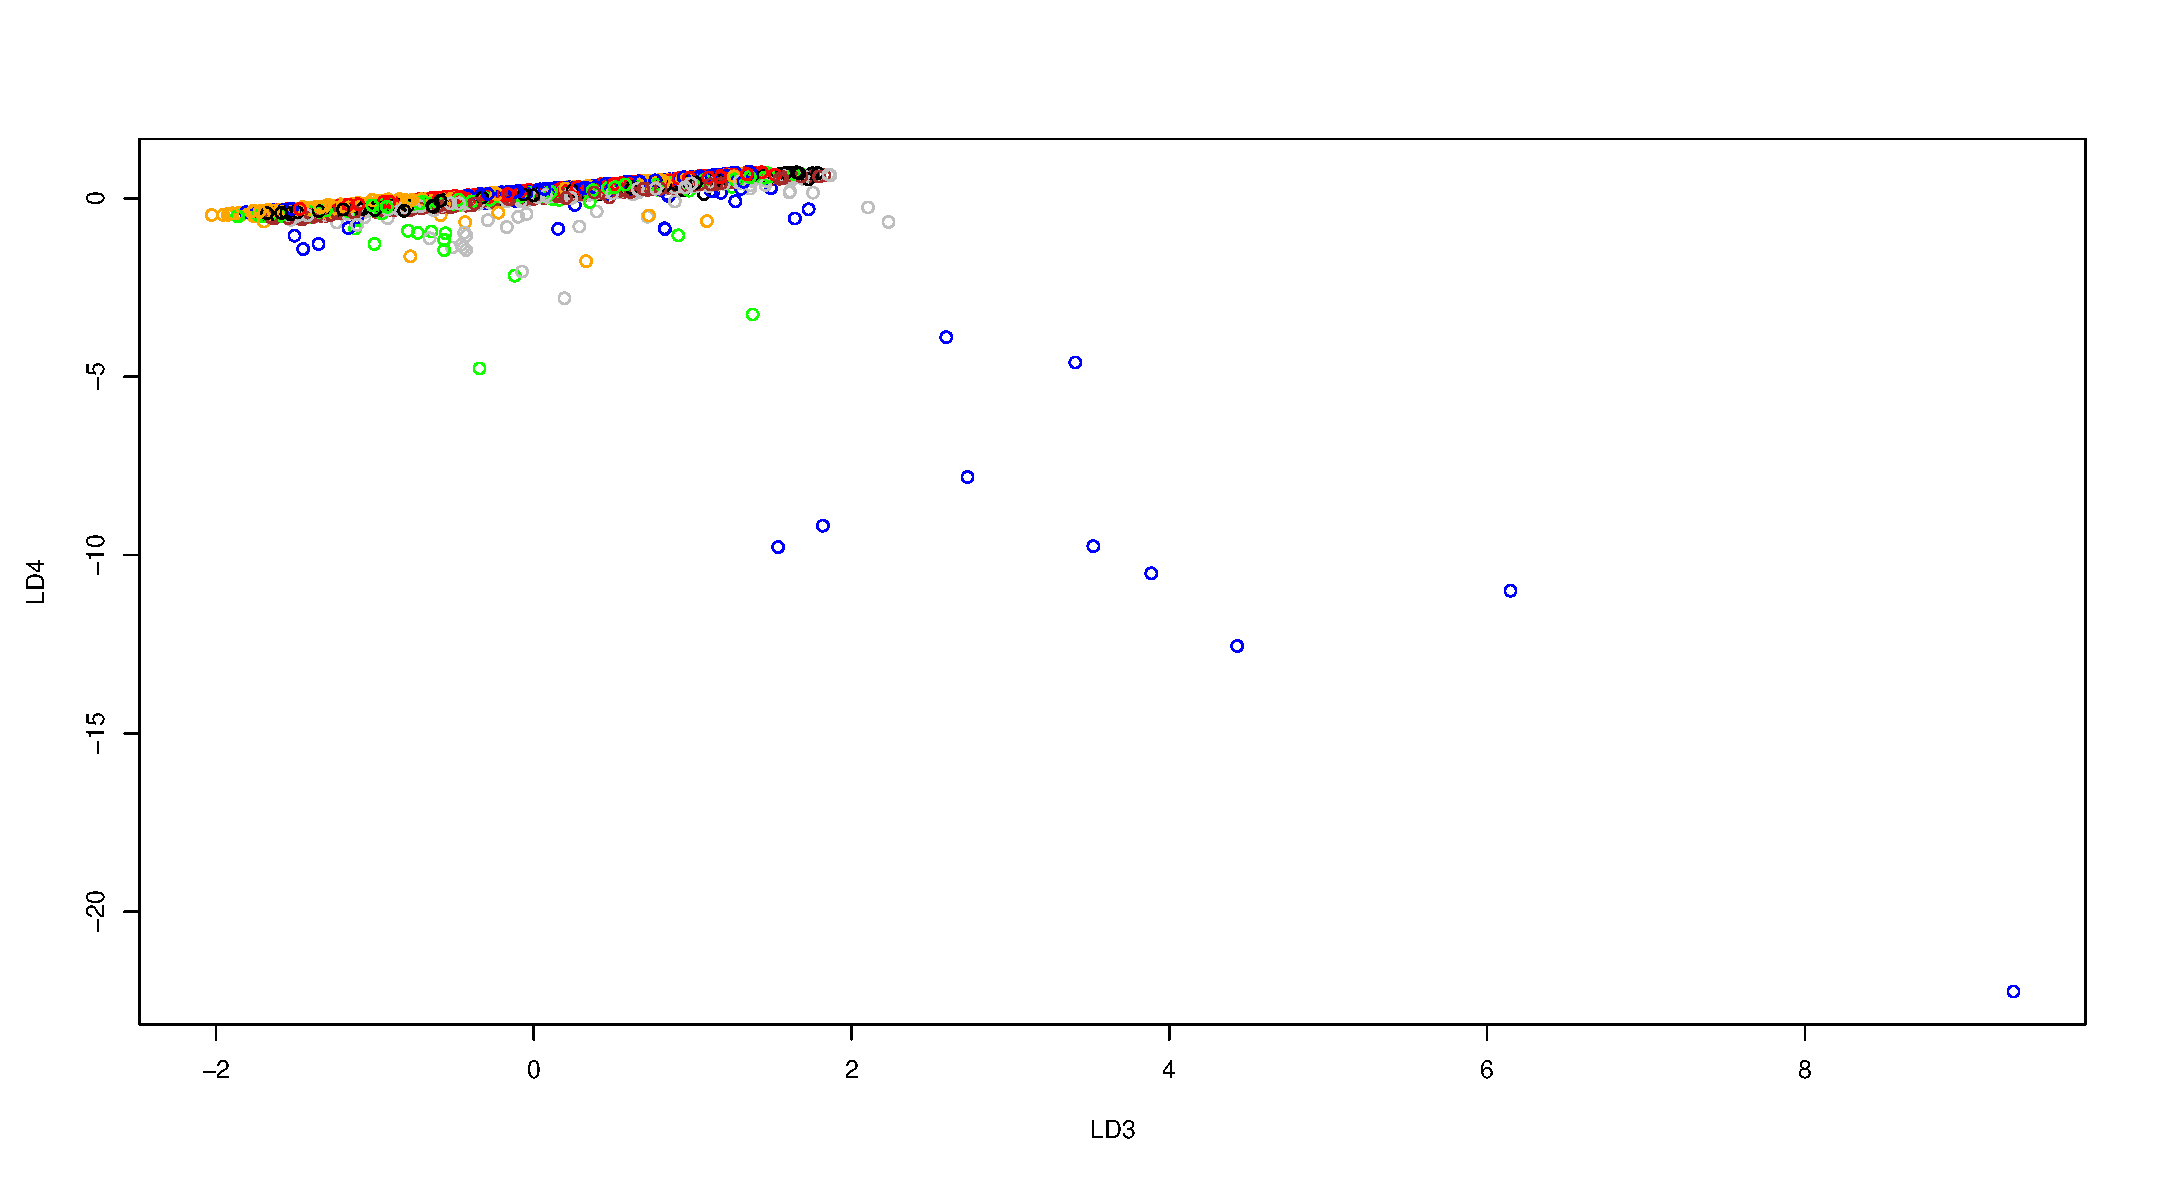
\includegraphics[width=12.1cm]{small_pcalda_LD34_train.eps}
\caption{\textit{Projection of PC space onto second two LD components space (small data set). Here, the colors represent different classes: red--brickface, brown--sky, 
blue--foliage, green--cement, orange--window, grey--path, black--grass.}}
\end{figure}


\subsection{Nonlinear Classifier}

Now, it's time for kernel PCA. By several experiments, the optimal parameter $\sigma$ in Gaussion kernel function is $\sigma=35.355$. 
The following table shows the result for the classifier:

\scalebox{0.88}{
 \begin{tabular}{|c|c|c|c|}
  \hline
  Size of Traing Set  & Number of KPCs & Acc. on Training Set & Acc. on Test Set \\ \hline
  $10\%$              & 105            & 0.9740260            & 0.7994228        \\ \hline
  $20\%$              & 146            & 0.9805195            & 0.8809524        \\ \hline
  $30\%$              & 180            & 0.9711400            & 0.8998145        \\ \hline
  $40\%$              & 199            & 0.9696970            & 0.9163059        \\ \hline
  $50\%$              & 205            & 0.9653680            & 0.9238095        \\ \hline
  $60\%$              & 214            & 0.9639250            & 0.9274892        \\ \hline
  $70\%$              & 223            & 0.9635127            & 0.9379509        \\ \hline
  $80\%$              & 227            & 0.9577922            & 0.9458874        \\ \hline
  $90\%$              & 230            & 0.9610390            & 0.9393939        \\ \hline
 \end{tabular}
}
 
Figure 8,9 shows the data projected on the first two and second two LD components space. As expected, the data processed by kernel PCA become much
more separated, as a result, building a classifier on this space becomes much easier, and the accuracy is much better.

\begin{figure}[htp]
\centering
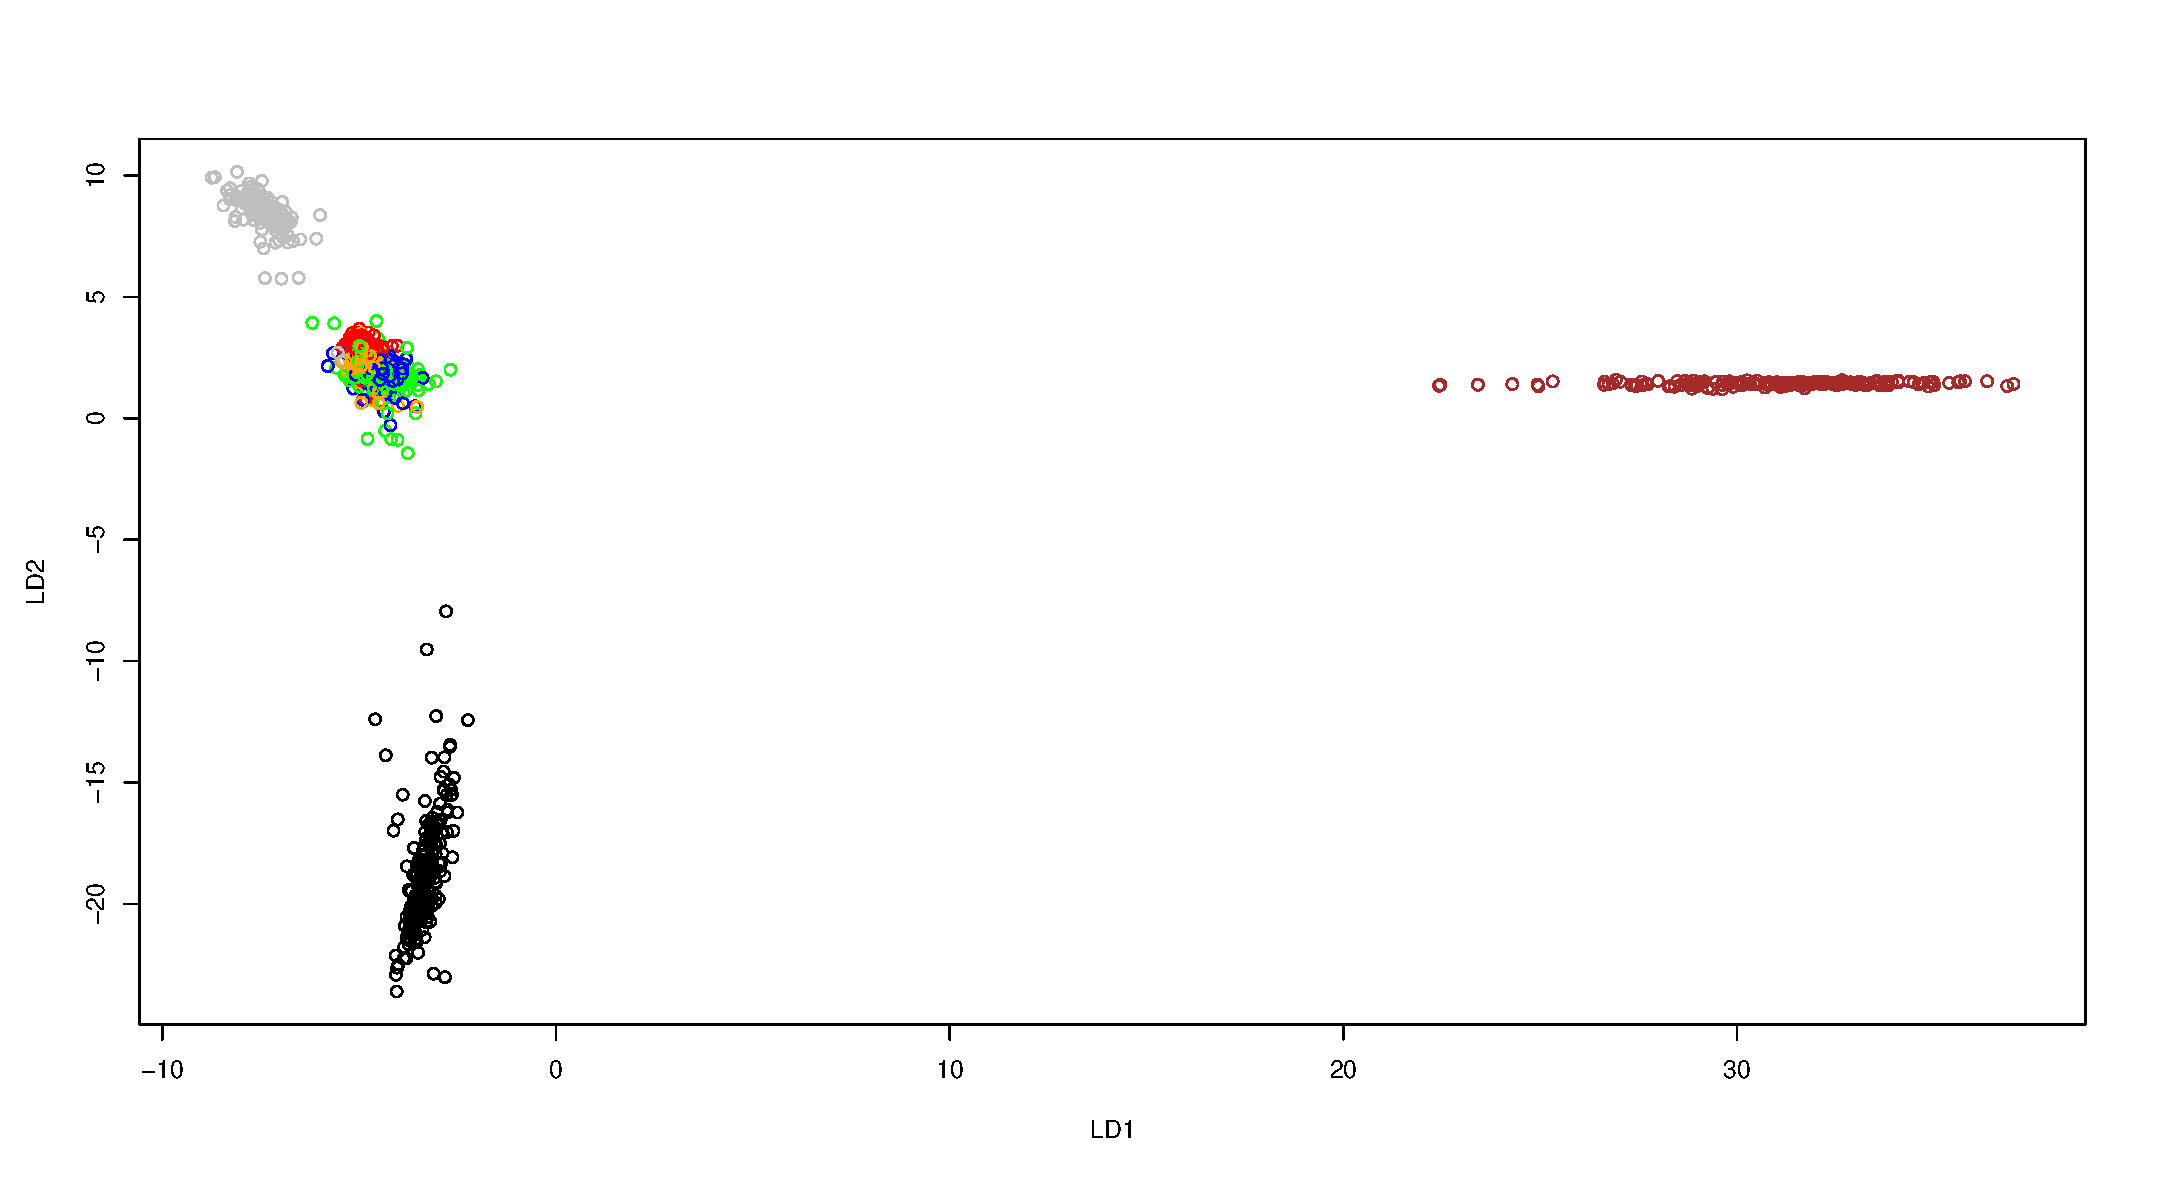
\includegraphics[width=12.1cm]{small_kpcalda_LD12_train.eps}
\caption{\textit{Projection of KPC space onto first two LD components space (small data set). Here, the colors represent different classes: red--brickface, brown--sky, 
blue--foliage, green--cement, orange--window, grey--path, black--grass.}}
\end{figure}

\begin{figure}[htp]
\centering
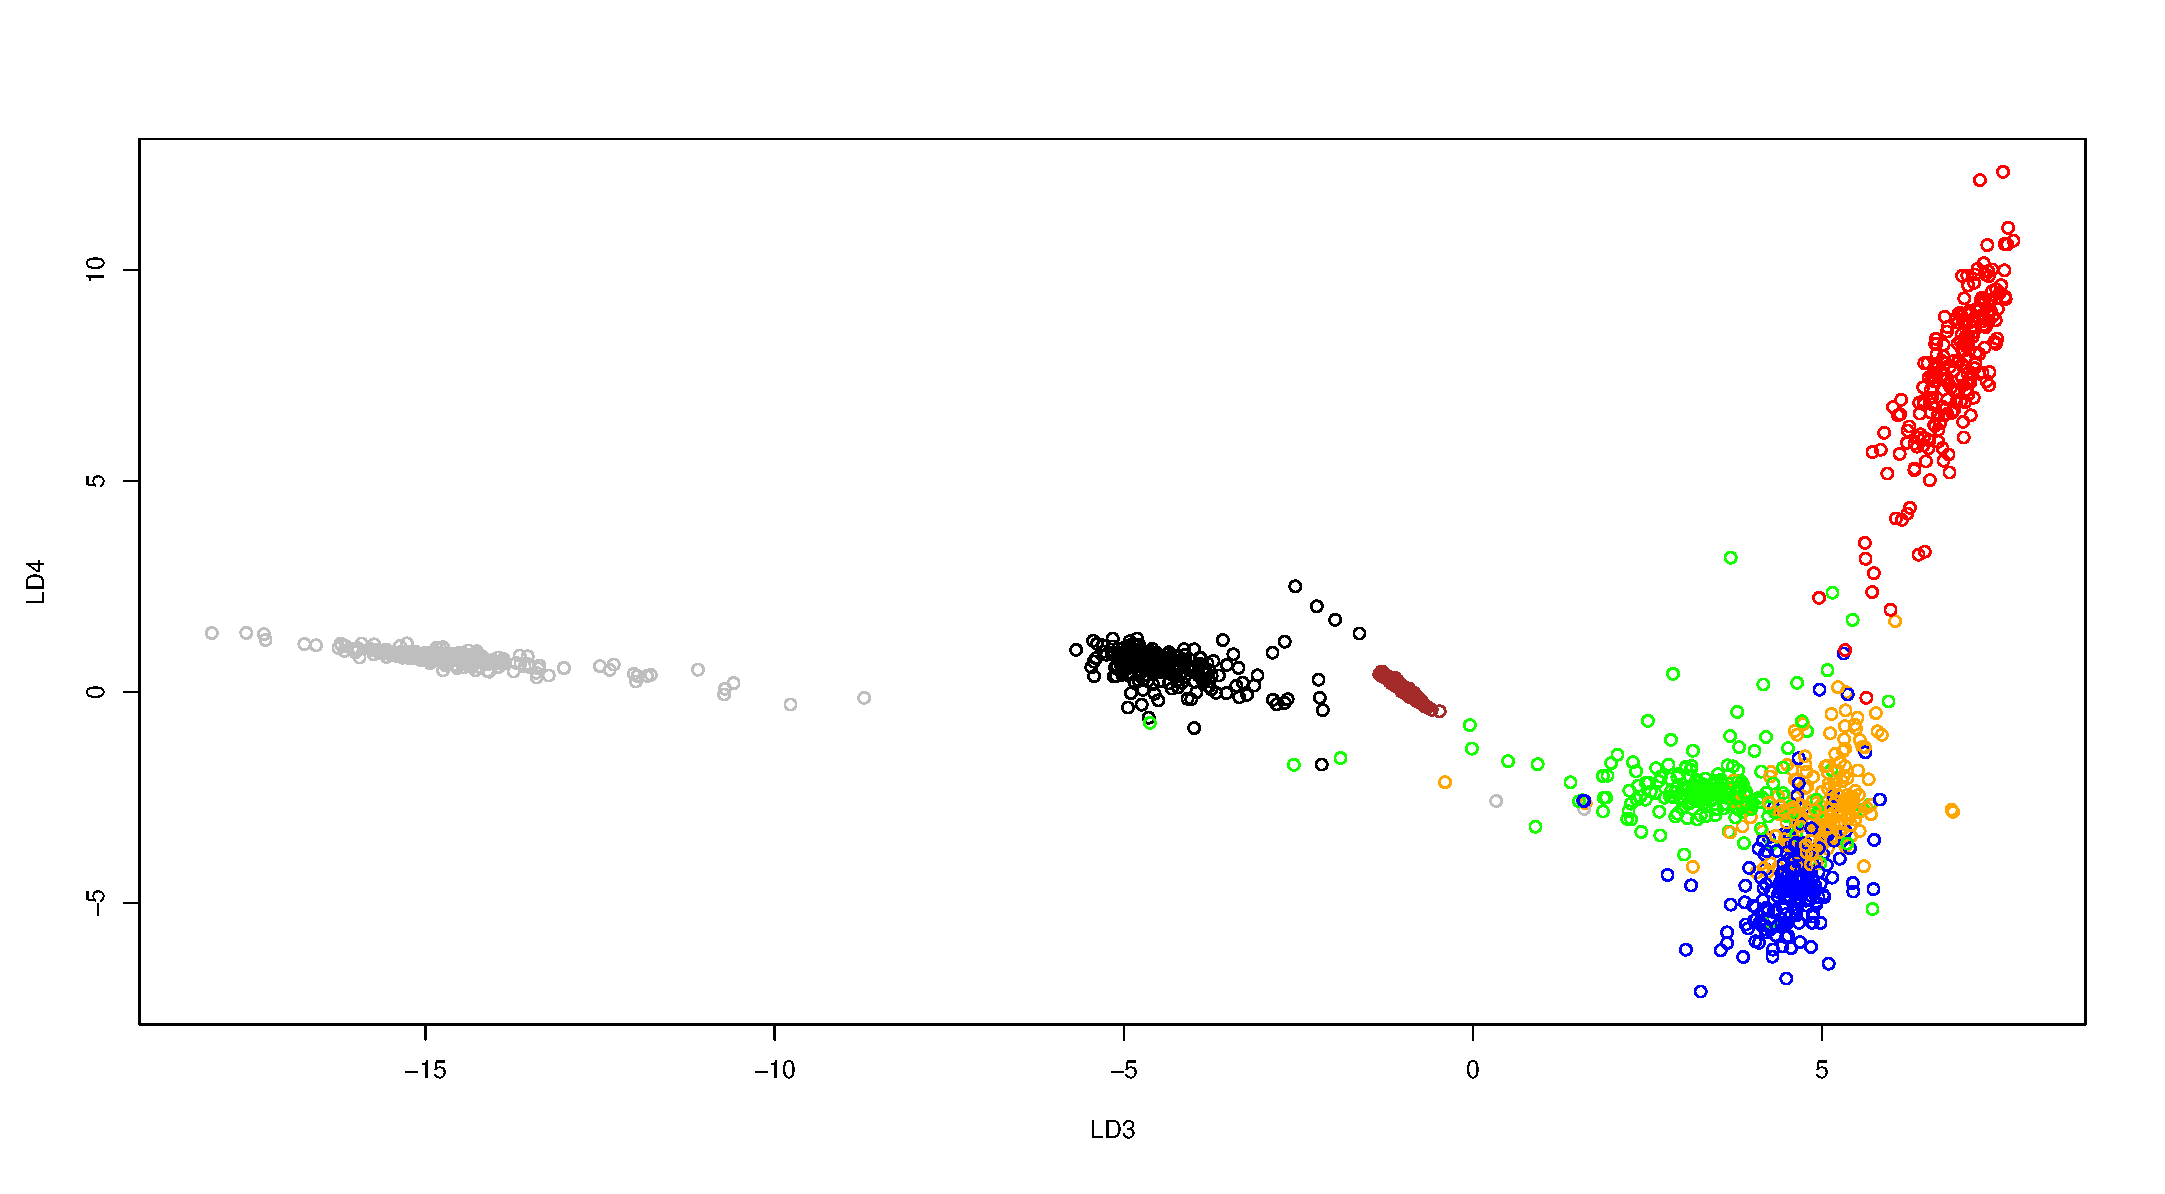
\includegraphics[width=12.1cm]{small_kpcalda_LD34_train.eps}
\caption{\textit{Projection of KPC space onto second two LD components space (small data set). Here, the colors represent different classes: red--brickface, brown--sky, 
blue--foliage, green--cement, orange--window, grey--path, black--grass.}}
\end{figure}


\end{document}


